While there are several proposals for a disaggregated \acrlong{wsc}, we will
use the Firebox\cite{firebox} project as an example throughout this thesis (see
Figure \ref{fig:fb_diagram}). The Firebox proposal incorporates ideas from
several academic and industrial projects and is representative of disaggregated
\glspl{wsc} in general.

\begin{figure}
    \centering
    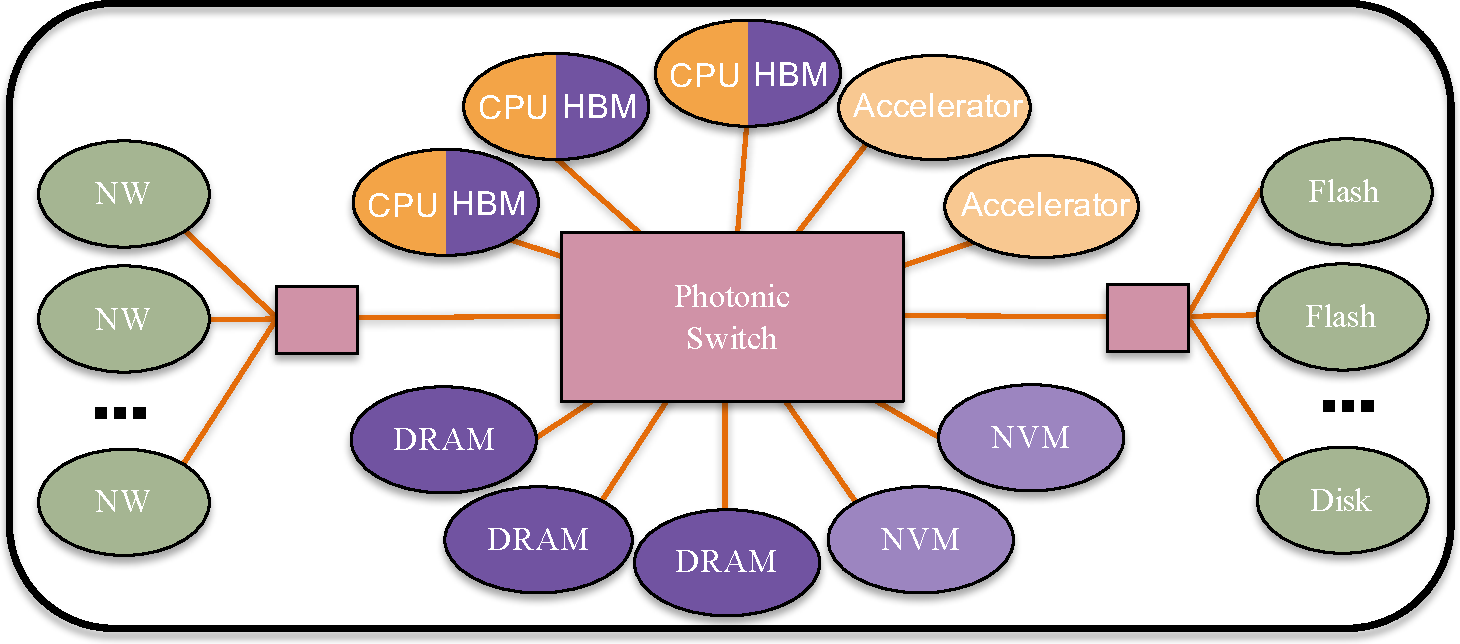
\includegraphics[width=0.9\columnwidth]{figs/FBDiagram.pdf} \label{fig:fb_diagram}
    \caption{The Firebox WSC proposal. Compute and memory resources become
    first-class citizens over a high-radix network, allowing flexible resource
    allocation and scaling. Lower-speed peripherals (such as disk or wide-area
    networking} can be connected farther away in the network topology.
\end{figure}

Firebox proposes using high-bandwidth, high-radix, networks to connect compute,
memory, and storage nodes in a \gls{wsc}. Firebox does not dictate any particular
networking technology, but is motivated by emerging integrated silicon photonic
network interfaces because they can be integrated directly on-die (or on
package, e.g., \gls{sip}), minimizing pin-out and providing high bandwidth at
low power. By multiplexing many wavelengths onto a single fiber (wave-division
multiplexing), it is possible to create a very high fanout while using few
physical interfaces. This fanout may enable very high radix switches that can
connect many SiPs within a single hop. Current estimates indicate these
photonic networks can achieve aggregate bandwidths exceeding
\SI{1}{\tera\bit\per\second} over 128 channels on a single
fiber\cite{naturePhotonic}\cite{Photonic09}. Link latencies (including photonic
transceiver crossings) are on the order of 10s of \si{\nano\second}, but final
latencies will be determined by protocol decisions. We believe round-trip
latencies (across a single switch) of approximately \SI{1}{\micro\second} to be
a conservative prediction. For reference, current infiniband EDR networks
provide approximately \SI{24}{\giga\bit\per\second} per link (with up to 12
links per NIC), and have round-trip latencies of approximately
\SI{2}{\micro\second}\cite{binnigNW}.

Compute nodes can be CPUs or special-purpose accelerators. In either case, they
will include some amount of high-bandwidth on-package memory (HBM), we
typically assume densities of approximately \SI{2}{\giga\byte} per core. This
on-package memory will have very high speed (up to
\SI{1}{\tera\byte\per\second}, at much lower power than traditional off-package
memories. A relatively large amount of on-package memory, coupled with very
fast networks allows most memory in the system to consist of network-attached memory
blades which are optimized for cost, power, and density. The total available
memory may be as much as \SI{1}{\peta\byte}. Other resources may also be used,
such as high-performance NAND flash, disks, and external network bridges.
Ultimately, the scale of such a system will be limited by network capacity, but
a Firebox would include at least thousands of cores and hundreds of
\si{\tera\byte} of bulk memory.

\paragraph{WSC Challenges}
\Glspl{wsc} promise to lower \gls{tco} significantly by improving utilization
and allowing components to develop and scale independently. These benefits
bring with them opportunities and challenges that bear mentioning. The
increased flexibility in resource allocation will require sophisticated and
scalable resource management algorithms that balance utilization, congestion,
and fairness. Encryption and authentication keys will also need to be managed
to protect memory traffic that is now exposed to attackers across the network.
In addition to being secure, memory-like interfaces must be very high
performance and any encryption or authentication mechanisms must match that
performance. Finally, this new heterogeneous memory hierarchy presents
challenges to applications and operating systems. What is the right interface
to expose the gap between local and remote memory? Will applications need to be
re-written to take advantage of it?
